\documentclass[12pt,oneside,openany,letterpaper]{article}


\usepackage{fancyhdr}
\usepackage{helvet}
\usepackage{amsmath}
%\usepackage{graphicx}
\usepackage[pdftex]{graphicx}
\usepackage{psfrag}
\usepackage{setspace}
%\usepackage[hypertex, linktocpage]{hyperref}[2003/11/30]
\usepackage[linktocpage]{hyperref}[2003/11/30]
\usepackage{lscape}
\usepackage{nicefrac}
\usepackage{mathrsfs}
\usepackage{units}
\usepackage{upgreek}
\usepackage{amssymb}
\usepackage{color}
\usepackage{wrapfig}
\usepackage{multirow}
\usepackage{url}
\usepackage{verbatim}
\usepackage{textcomp}
\usepackage{epstopdf}
\usepackage{enumitem}


\onehalfspacing \setlength\textheight{667pt}
\setlength\textwidth{506pt} \setlength\oddsidemargin{-18pt}
\setlength\topmargin{-20pt}
%\setlength\footskip{24pt}
\addtolength\headheight{2.5pt} \addtolength\headsep{-14pt}
%\fancyhead[R]{\includegraphics[height=10.5pt]{ubclogo_bw.eps}\#:  55907968}
%\renewcommand\familydefault{\sfdefault}
\pagestyle{empty}

\newenvironment{packed_enum}{
\begin{enumerate}
  \setlength{\itemsep}{0pt}
  \setlength{\parskip}{0pt}
  \setlength{\parsep}{0pt}
}{\end{enumerate}}



\fancyhead[L]{\emph{Introduction to Electronics}}\fancyhead[R]{$LRC$ Transients and Resonance}
\fancyfoot[L]{PHYS 231}\fancyfoot[R]{Experiment 1}
\pagestyle{fancy} \pagenumbering{arabic}

\begin{document}
\thispagestyle{plain}
\begin{center}
{\large{\bf{\fontfamily{phv}\selectfont Physics 231 - Introduction to Laboratory Electronics (Exp.~1)}}}
\end{center}

\noindent The purpose of this experiment is to gain familiarity with the equipment you will use in many of the subsequent experiments. This will involve performing a number of simple measurements with an oscilloscope and digital multimeters (DMM's).

~


{\bf Part 1 - Instrument specifications}

~

\noindent Links to information and specifications for the equipment you will use are provided on the course website: \href{http://cmps-people.ok.ubc.ca/jbobowsk/phys231calendar.html}{http://cmps-people.ok.ubc.ca/jbobowsk/phys231calendar.html}. Find the following information and record it in your lab book:

\begin{enumerate}[label=\alph*)]
\item The input impedances of the oscilloscope and both DMM's (operating in DC voltmeter mode).
\item The AC (alternating current) frequency ranges over which both of the DMM's operate when in voltmeter mode.
\end{enumerate}


{\bf Part 2 - Introduction to the oscilloscope and function generator}

~

\noindent You should take some time to explore all of the controls on the oscilloscope and function generator -- the following points will provide some guidance in getting started with these instruments.

\begin{enumerate}[label=\alph*)]
\item Connect the output of the {\bf function generator} to one of the channel inputs of the oscilloscope and set the generator frequency to some low value near $100\rm\ Hz$ and to a sinusoidal output. Obtain a stable pattern by adjusting the trigger control of the oscilloscope. First, set the {\bf TRIGGER Type} to {\bf Edge} and the {\bf TRIGGER Mode} to {\bf Normal} and set the {\bf TRIGGER Source} to {\bf AC Line}. You should see the waveform but it will start sweeping at apparently random times because the oscilloscope is being triggered by the $60\rm\ Hz$ oscillation in the power lines. If the {\bf TRIGGER Source} is set to the same channel being used for the channel input, then triggering will be synchronized with the signal form the generator. Try varying the {\bf TRIGGER Level} and the {\bf TRIGGER Slope} and observe how the phase of the waveform varies on the oscilloscope screen. Also, observe the effect of increasing the frequency of the signal from the function generator and changing the waveform form from sinusoidal to triangular or square wave.
\item Record the effects on the oscilloscope waveform when you vary the vertical and horizontal positions and sweep rate (sec/div).
\item Two channel operation: Set the function generator to $1\rm\ kHz$ and connect the {\bf TTL} output of the function generator to the ``CH 1'' input of the oscilloscope and the signal output of the function generator to ``CH 2''. Set the {\bf TRIGGER Source} to {\bf CH 1}. The waveforms of both signals should now be visible on the oscilloscope. For both sinusoidal and triangular waveforms, vary the signal amplitude and frequency and compare their effects on the two waveforms visible on the oscilloscope. Explain why the {\bf TTL} output of the generator is useful as a triggering source and try this out by moving the {\bf TTL} output to the {\bf External Trigger} input of the oscilloscope (the {\bf TRIGGER Source} should then be set to {\bf Ext}).
\item Use the cursor functions on the oscilloscope to measure the amplitude of the {\bf TTL} output as well as its period.
\item With the signal output in CH 1 and the {\bf TTL} output in CH 2, in the {\bf TRIG MENU}, try setting {\bf TRIGGER Mode} to both {\bf Auto} and {\bf Normal}. Figure out what the difference is (hint: see what happens if CH 1 input signal is disconnected and the {\bf TRIGGER Source} is set to {\bf CH 1}.)
\end{enumerate}

~


{\bf Part 3 - The digital multimeters}

~

\begin{enumerate}[label=\alph*)]
\item Using the DMM, measure the resistances of two resistors and compare the results with the values indicated on them by the resistor colour code.  Both the DMM measurements and the values obtained from the colour code should have an associated uncertainty.
\item When set for {\bf AC operation}, the DMM’s are designed to display the {\bf true rms} value of the input signal, regardless of the shape of the waveform selected. Using both a DMM and the oscilloscope connected in parallel to measure the signal generated by the function generator (with frequency set at some intermediate value, say $1\rm\ kHz$), compare the reading on the DMM with the amplitude observed on the oscilloscope for a sine wave, a square wave, and a triangular wave. For the sine wave and square wave show that these measurements are in agreement with the definition of rms. Root-Mean-Square is the square root of the mean of the square of the waveform: 
\begin{equation}
V_\mathrm{rms} = \sqrt{\overline{v^2(t)}}.
\end{equation}
\end{enumerate}

\clearpage

{\bf Important Note:}

~

\noindent In subsequent experiments, be very careful with your {\bf ground connections}. It is a good rule to connect all grounds at {\bf only one point} in the circuit! Otherwise, you run the risk of ``shorting out'' some of the components of the circuit via the ground connections. The examples depicted below show a series combination of two components $Z_1$ and $Z_2$.  These components could be resistors, capacitors, or inductors (or any combination of these).  Suppose we wanted to view the waveforms across both $Z_1$ and $Z_2$ on the two channels of the oscilloscope.  Figure~\ref{fig:fig1} shows a set up that, at first glance, seems like it would do the job.
\begin{figure}[h!]
\begin{center}
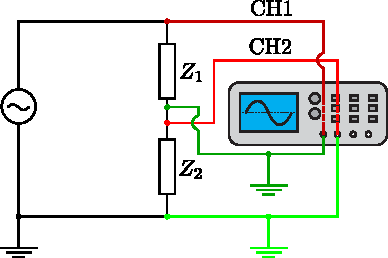
\includegraphics[width=.5\textwidth]{figures/Lab1Fig1.pdf}\caption{\label{fig:fig1}An incorrect experimental set up.  The ground connections on either side of $Z_2$ short circuit this component.  CH2 of the oscilloscope will  display a constant of zero volts.}
\end{center}
\end{figure}

\noindent The issue with his set up is that the outer conductors of the oscilloscope are permanently connected to ground (zero volts).  One of the function generator output terminals is also connected to ground.  To properly probe your circuit, all of the grounds need to be connected to a common point or node in the circuit.

\clearpage

\noindent Figure~\ref{fig:fig2} shows a proper set up in which all of the grounds are connected at a common point. Notice that, in this case, CH2 is measuring the voltage across $Z_2$ and CH1 is measuring the voltage across the series combination of $Z_1 + Z_2$ (or, equivalently, the output of the function generator).  With the oscilloscopes that we're using, it is not possible to directly measure the voltages $Z_1$ and $Z_2$ on CH1 and CH2, respectively.  However, the oscilloscope has a {\bf MATH} menu that allows us to display $\mathrm{CH1} - \mathrm{CH2}$ and, hence, the voltage across $Z_1$.  We'll use the oscilloscope in exactly with way in Experiment \#2.

\begin{figure}[h!]
\begin{center}
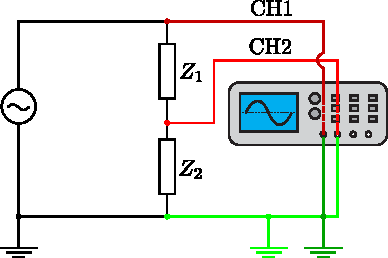
\includegraphics[width=.5\textwidth]{figures/Lab1Fig2.pdf}\caption{\label{fig:fig2}An incorrect experimental set up.  The ground connections on either side of $Z_2$ short circuit this component.  CH2 of the oscilloscope will  display a constant of zero volts.}
\end{center}
\end{figure}


\end{document}
